\section{gRPC - Remote Call Procedure}
\begin{multicols*}{2}
    \begin{itemize}
        \item Neue Standard-Technologie für Backend-Kommunikation in .NET
        \item Primär Server-to-Server Kommunikation im Fokus
        \item In fast allen verteilten Systemen (Distributed Systems) verwendet
        \item Hohe Performance von zentraler Bedeutung
        \item Nicht als Frontend-API gedacht
    \end{itemize}
\fat{Grundprinzipien:}
\begin{itemize}
    \item Einfache Service-Definition
    \item Sprach-Unabhängigkeit
    \item Problemlose Skalierbarkeit
    \item Bi-direktionales Streaming
    \item Integrierte Authentisierungsmechanismen
    \item Kommunikation über HTTP/2
\end{itemize}
\subsection{Architektur}
gRPC ist ein Software Development Kit (SDK), welches in Visual Studio (Code) integriert ist.
\subsubsection{Beispiel}
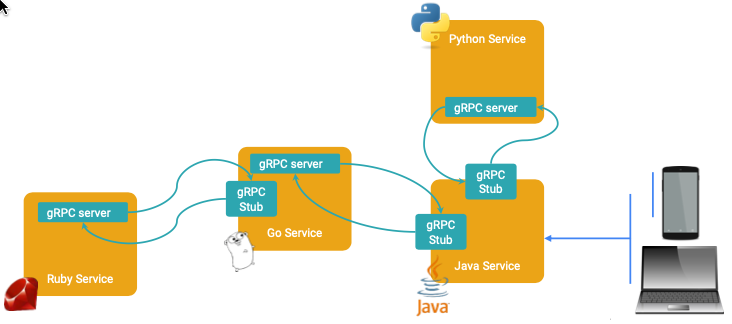
\includegraphics[width=\columnwidth]{rpcex}
\subsubsection{Aufbau inkl. Kommunikation}
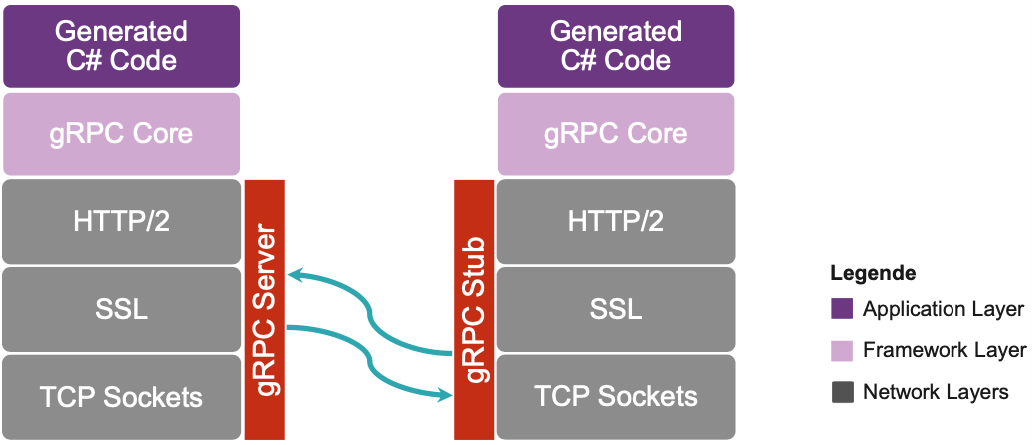
\includegraphics[width=\columnwidth]{aufbau}
\subsubsection{RPC vs. REST}
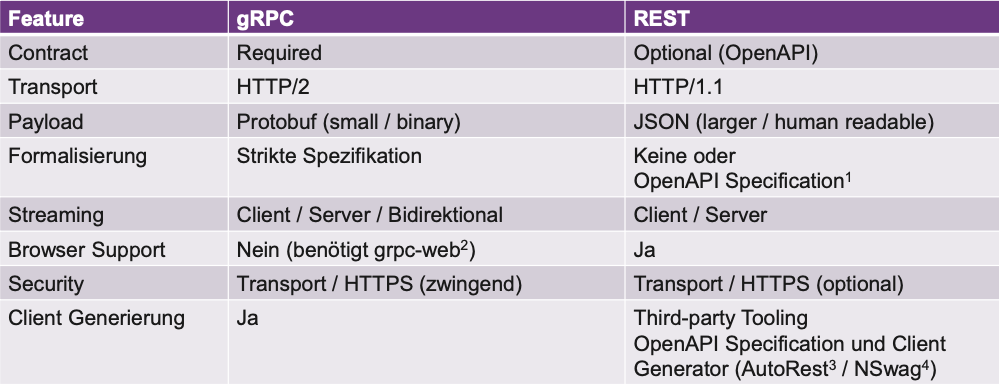
\includegraphics[width=\columnwidth]{rpcrest}
\subsubsection{HTTP/2}
\begin{itemize}
    \item Multiplexing
    \begin{itemize}
        \item Mehrere gRPC Calls pro TCP/IP Connection
        \item Massiv kleinerer Overhead für Disconnect / Reconnect (kleinere Latency)
    \end{itemize}
\end{itemize}
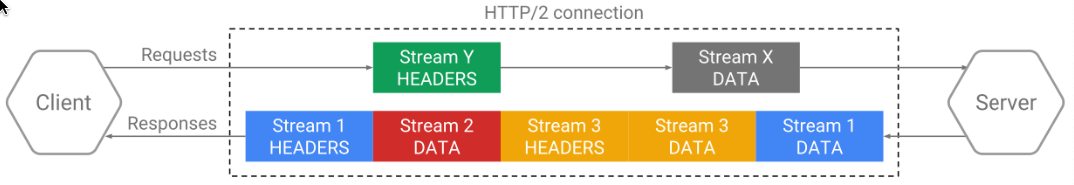
\includegraphics[width=\columnwidth]{asynchttp}
\begin{itemize}
    \item Bidirectional Streaming
    \begin{itemize}
        \item Asynchrones, Nicht-blockierendes Senden und Empfangen von Streams
        \item Senden und Empfangen parallel möglich
    \end{itemize}
    \item Basiert auf HTTPS
    \item HTTP Header werden standardmässig komprimiert
\end{itemize}
\subsubsection{Beispiel Service}
\fat{Definition eines Services} unter Verwendung der Interface Definition Language
\begin{lstlisting}
syntax = "proto3";
option csharp_namespace = "BasicExample"; 
package Greet;

// Service definition
service Greeter {
    // Sends a greeting
    rpc SayHello (HelloRequest)
    returns (HelloReply);
}

// Request message containing the user's name
message HelloRequest {
    string name = 1;
}

// Response message containing the greetings
message HelloReply {
    string message = 1;
}
\end{lstlisting}
\fat{Implementation des Services}
\begin{lstlisting}
//Erben von der Definitionsklasse
public class GreeterService : Greeter.GreeterBase {

    //Überschreiben der Methode HelloReply
    public override Task<HelloReply> SayHello(
        HelloRequest request, 
        ServerCallContext context)
        => Task.FromResult(new HelloReply
        {
            Message = "Hello " + request.Name
        });
}
\end{lstlisting}
\subsubsection{Beispiel Client}
\begin{lstlisting}
// The port number(5001) must match the port of the gRPC server.
GrpcChannel channel = GrpcChannel.ForAddress("https://localhost:5001");
Greeter.GreeterClient client = new(channel); //Generierter Client Stub

HelloReply reply = await client.SayHelloAsync(
    new HelloRequest { Name = "GreeterClient" } //Remote Procedure Call
);
Console.WriteLine(\$"Greeting: {reply.Message}");
\end{lstlisting}

\subsection{Protocol Buffers}
\begin{itemize}
    \item Benutzt \fat{Interface Definition Language (IDL)} (eine Subform einer Domain Specific Language (DSL)),
    welche ein Service Interface platform- und sprachneutral beschreibt.
    \item \fat{DataModel:} Beschreibt Messages resp. Request- und Response-Objekte
    \item \fat{WireFormat:} Beschreibt das Binärformat zur Übertragung
    \item Serialisierungs-/Deserialisierungs-Mechanismen
    \item Service-Versionierung
\end{itemize}
\subsubsection{Value Types}
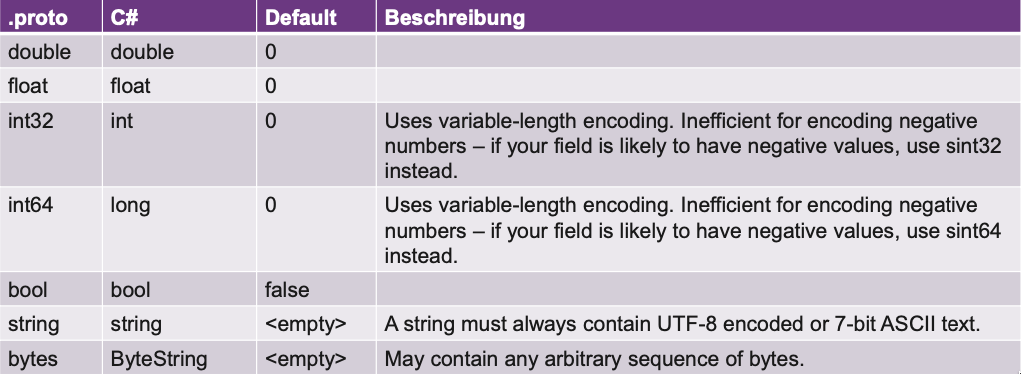
\includegraphics[width=\columnwidth]{protovaluetypes}
\subsubsection{Proto Files}    
\begin{itemize}
    \item Datei-Endung *.proto
    \item Header
    \begin{itemize}
        \item Allgemeine Definitionen (syntax, option, etc.)
    \end{itemize}
    \item Services
    \begin{itemize}
        \item 0 oder mehr Services
        \item 1 oder mehr Service-Methoden pro Service
        \item Service-Methoden haben immer genau 1 Parameter und 1 Rückgabewert
    \end{itemize}
    \item Message Types
    \begin{itemize}
        \item 1 oder mehr Fields
        \item Field definiert sich aus: Type, Unique Name, Unique Field Number (Versionierung)
    \end{itemize}
\end{itemize}
\begin{lstlisting}
syntax = "proto3";
option csharp_namespace = "_01_BasicExample"; 

package Greet;
// Service definition
service Greeter {
    // Sends a greeting
    rpc SayHello (HelloRequest)
        returns (HelloReply);
}
// Request message containing the user's name
message HelloRequest {
    string name = 1;
}
// Response message containing the greetings
message HelloReply {
    string message = 1;
}
\end{lstlisting}
\fat{Null-Werte / Leere Message:} 
\begin{lstlisting}
import "google/protobuf/empty.proto";
...
service Greeter {
    // Sends a greeting
    rpc SayHello (HelloRequest)
        returns (google.protobuf.Empty);
}
\end{lstlisting}
\subsubsection{Messages / Fields}
\fat{Singular Fields:}
\begin{itemize}
    \item Angabe des Feldtypen
    \begin{itemize}
        \item Skalarer Werttyp
        \item Anderer Message Type
        \item Enumeration
    \end{itemize}
    \item Unique Field Name
    \begin{itemize}
        \item Wird für Generatoren von C\# Klassen verwendet
        \item Lower Snake Case (Underscores)
    \end{itemize}
    \item Unique Field Number
    \begin{itemize}
        \item Identifikator für das Binärformat
        \item $1$-$536'870'911$ ohne $19'000$ und $19'999$
    \end{itemize}
\end{itemize}
\begin{lstlisting}
message SearchRequest { 
    string query = 1;
    int32 page_number = 2; 
    int32 result_per_page = 3;
}   
\end{lstlisting}
\fat{Repeated Fields:}
\begin{itemize}
    \item Liste von Werten
    \item Schlüsselwort ''repeated''
    \item Ergibt eine Liste von Strings
\end{itemize}
\begin{lstlisting}
message SearchResponse {
    repeated string results = 1;
}
\end{lstlisting}
\fat{Enumerationen:}
\begin{itemize}
    \item Analog Enumerationstypen in .NET
    \item Definition innerhalb einer Message oder im Proto-File Root
    \item Enum-Member mit Wert 0 muss zwingend existieren (Default Value)
    \item Schlüsselwort ''reserved'' kann auch für Enumerations verwendet werden
\end{itemize}
\begin{lstlisting}
message SearchRequest { 
    Color searchColor = 1; 
    Size searchSize = 2;
    
    //Definition innerhalb Message
    enum Color {
        RED = 0; // 0 must exist
        GREEN = 1;
    }
}

//Definition im Proto-File Root
enum Size {
    S = 0; // 0 must exist 
    M = 1;
    L = 2;
}
\end{lstlisting}
\subsubsection{Aufteilen von proto files}
Auf Inhalt von anderen Proto files kann über ein import statement zugegriffen werden.
Andere Message Types können ebenfalls als fields benutzt werden.
\begin{lstlisting}
// File: example.proto
import "protos/_base.proto";

message Search {
    Query query = 1;
    LogicalOperator operator = 2;
}

message Query {
    string filter = 1;
}

// File: _base.proto
enum LogicalOperator {
    AND = 0;
    OR = 1;
    XOR = 2; 
}
\end{lstlisting}
\subsubsection{Reserved Fields}
\begin{itemize}
    \item Für Versionierung gedacht
    \item Wiederverwendung wird vom Protocol Buffer Compiler verhindert
    \item Schlüsselwort ''reserved'' bei: Unique Field Name, Unique Field Number
\end{itemize}
\begin{lstlisting}
message SearchRequest { 
    reserved 1, 3, 20 to 30; 
    reserved "page_number", "result_per_page";

string query = 1; // Compilerfehler
int32 page_number = 2; // Compilerfehler
int32 result_per_page = 3; // Compilerfehler
}

//Reservieren eines Ranges
reserved 1 to 3
\end{lstlisting}

\subsection{gRPC C\# API}
\subsubsection{Protocol Buffer Compiler}
\begin{itemize}
    \item protoc.exe mit Plugins für C\# Code Generierung
    \item Automatisch in Build Pipeline eingebunden
    \item NuGetPackage: Grpc.Tools
    \item Proto-Compiler Output in ''obj'' Folder
\end{itemize}
\fat{Aufbau Server Projekt:}
\begin{lstlisting}
<Project Sdk="Microsoft.NET.Sdk.Web"> 
<PropertyGroup>
    <TargetFramework>netcoreapp3.0</TargetFramework>
    <RootNamespace>BasicExample</RootNamespace> 
</PropertyGroup>
<ItemGroup>
    <None Remove="Protos\greet.proto" />
</ItemGroup>
<ItemGroup>
    //Protobuf Include
    <Protobuf Include="Protos\greet.proto" 
        GrpcServices="Server"> //Zu generierende Klassen
        <Link>Protos\greet.proto</Link> //File Link
    </Protobuf> 
</ItemGroup>
<ItemGroup>
    //Server als AspNetCore Server
    <PackageReference Include="Grpc.AspNetCore" Version="..." />
</ItemGroup>
</Project>
\end{lstlisting}
\fat{Aufbau Client Projekt:}
\begin{lstlisting}
<Project Sdk="Microsoft.NET.Sdk"> 
<PropertyGroup>
    <OutputType>Exe</OutputType> 
    <TargetFramework>netcoreapp3.0</TargetFramework> 
    <RootNamespace>BasicExampleClient</RootNamespace>
</PropertyGroup>
<ItemGroup>
    //Relative Pfad zu Protofile in Server-Projekt
    <Protobuf Include="..\<relative_path>\greet.proto"
        GrpcServices="Client"> //Zu generierende Klasse
        <Link>Protos\greet.proto</Link>
    </Protobuf>
</ItemGroup>
<ItemGroup>
    <PackageReference Include="Google.Protobuf" Version="..." /> 
    <PackageReference Include="Grpc.Net.Client" Version="..." /> 
    <PackageReference Include="Grpc.Tools" Version="...">[...] </PackageReference>
</ItemGroup>
</Project>
\end{lstlisting}
\subsubsection{Generierter Code}
\fat{Namespace:}
\begin{lstlisting}
//Proto-File
option csharp_namespace = "ProtocolBufferRunningExamples"; 

//C# Output
namespace ProtocolBufferRunningExamples 
\end{lstlisting}
\fat{Abstrakte Basisklasse:} Pro Service wird eine abstrakte Basisklasse erzeugt.
Muss beachtet werden wenn Service implementiert wird! Siehe Beispiel auf erster Seite des Themas.
\begin{lstlisting}
public class GreeterService : Greeter.GreeterBase
\end{lstlisting}
\begin{lstlisting}
//Proto-File
service MyCustomerService { /* ... */ }

//C# Output
public static partial class MyCustomerService {
    public abstract partial class MyCustomerServiceBase { /* ... */ }
}
\end{lstlisting}
\fat{Registration des Service beim Startup:}
 \begin{lstlisting}
WebApplicationBuilder builder = WebApplication.CreateBuilder(args);

//Registrierung der gRPC Types via Dependency Injection
// Add services to the container.
builder.Services.AddGrpc();

WebApplication app = builder.Build(); 

//Definition der Endpoints, einmal pro Service
// Configure the HTTP request pipeline.
app.MapGrpcService<GreeterService>();

app.Run();
\end{lstlisting}
\subsection{C\# API Beispiel: Customer Service}
\subsubsection{Aufbau}
\begin{multicols*}{2}
    \fat{\normalsize CustomerService}\\
    RPC GetCustomers
    \begin{itemize}
        \item Input: <None>
        \item Output: Liste der Kunden ohne Bestellungen
    \end{itemize}
    RPC GetCustomer
    \begin{itemize}
        \item Input: ID Filter / Include Orders (true/false)
        \item Output: Kunde mit oder ohne Bestellungen
    \end{itemize}
\columnbreak
\fat{\normalsize OrderService}\\
RPC GetOrders
    \begin{itemize}
        \item Input: Customer ID Filter
        \item Output: Liste der Bestellungen zum Kunden
    \end{itemize}
\end{multicols*}
\subsubsection{Proto Files}
\begin{lstlisting}
syntax = "proto3";

option csharp_namespace = "ProtocolBufferRunningExamples";

import "google/protobuf/empty.proto";

package Services;

service CustomerService {
                     //<None> Parameter
    rpc GetCustomers (google.protobuf.Empty) 
        returns (GetCustomersResponse);
    rpc GetCustomer (GetCustomerRequest) 
        returns (GetCustomerResponse);
}
service OrderService {
    rpc GetOrders (GetOrdersRequest) 
        returns (GetOrdersResponse);
}

// --- Customer types ---
message GetCustomersResponse {
    repeated CustomerResponse data = 1;
}

message GetCustomerResponse { CustomerResponse data = 1; }

message GetCustomerRequest {
    int32 id_filter = 1; bool include_orders = 2; 
}

message CustomerResponse {
    int32 id = 1;
    string first_name = 2;
    string last_name = 3;
    Gender gender = 4;

    repeated OrderResponse orders = 10;
}

enum Gender {
    UNKNOWN = 0; FEMALE = 1; MALE = 2; OTHER = 3;
}

// --- Order types ---
message GetOrdersRequest { int32 customer_id_filter = 1; }

message GetOrdersResponse {
    repeated OrderResponse data = 1;
}

message OrderResponse {
    string product_name = 1;
    int32 quantity = 2;
    double price = 3;
}
\end{lstlisting}
\subsubsection{Service Implementation}
\fat{CustomerService}
\begin{lstlisting}
namespace ProtocolBufferRunningExamples.Services;

public class MyCustomerService : CustomerService.CustomerServiceBase
{
    public override Task<GetCustomersResponse> GetCustomers(Empty request, ServerCallContext context)
    {
        GetCustomersResponse response = new();
        response.Data.AddRange(MockData.Customers);

        return Task.FromResult(response);
    }

    public override Task<GetCustomerResponse> GetCustomer(GetCustomerRequest request, ServerCallContext context)
    {
        CustomerResponse[] data = request.IncludeOrders
            ? MockData.CustomersWithOrders
            : MockData.Customers;

        GetCustomerResponse response = new()
        {
            Data = data.Single(c => c.Id == request.IdFilter)
        };

        return Task.FromResult(response);
    }
}
\end{lstlisting}
\fat{OrderService}
\begin{lstlisting}
namespace ProtocolBufferRunningExamples.Services;

public class MyOrderService : OrderService.OrderServiceBase
{
    public override Task<GetOrdersResponse> GetOrders(GetOrdersRequest request, ServerCallContext context)
    {
        GetOrdersResponse response = new();

        IEnumerable<OrderResponse> dataFiltered = MockData
            .Orders[request.CustomerIdFilter];

        response.Data.AddRange(dataFiltered);

        return Task.FromResult(response);
    }
}
\end{lstlisting}
\subsubsection{Client Implementation}
\fat{Customer}
\begin{lstlisting}
// The port number (5001) must match the port of the gRPC server.
GrpcChannel channel = GrpcChannel.ForAddress("https://localhost:5001");

// Customer service calls
CustomerService.CustomerServiceClient customerClient = new(channel);

Empty request1 = new();
GetCustomersResponse response1 = await customerClient.GetCustomersAsync(request1); 
Console.WriteLine(response1);

GetCustomerRequest request2 = new() { IdFilter = 1 };
GetCustomerResponse response2 = await customerClient.GetCustomerAsync(request2); 
Console.WriteLine(response2);

request2.IncludeOrders = false;
response2 = await customerClient.GetCustomerAsync(request2);
Console.WriteLine(response2);
\end{lstlisting}
\fat{Order}
\begin{lstlisting}
// The port number (5001) must match the port of the gRPC server.
GrpcChannel channel = GrpcChannel.ForAddress("https://localhost:5001");

// Order service calls
OrderService.OrderServiceClient orderClient = new(channel);

GetOrdersRequest request3 = new() { CustomerIdFilter = 1 }; 
GetOrdersResponse response3 = await orderClient.GetOrdersAsync(request3); 
Console.WriteLine(response3);
\end{lstlisting}

\subsection{Streams}
Reliability:
\begin{itemize}
    \item End-to-end Reliability: Garantiertes Ausliefern der Nachrichten gewährleistet
    \item Ordered Delivery: Reihenfolge gewährleistet
\end{itemize}
Schlüsselwort ''stream'' vor Typbezeichnung signalisiert RPC, dass dieses Ergebnis nicht synchron, sondern gestreamt übertragen werden kann.
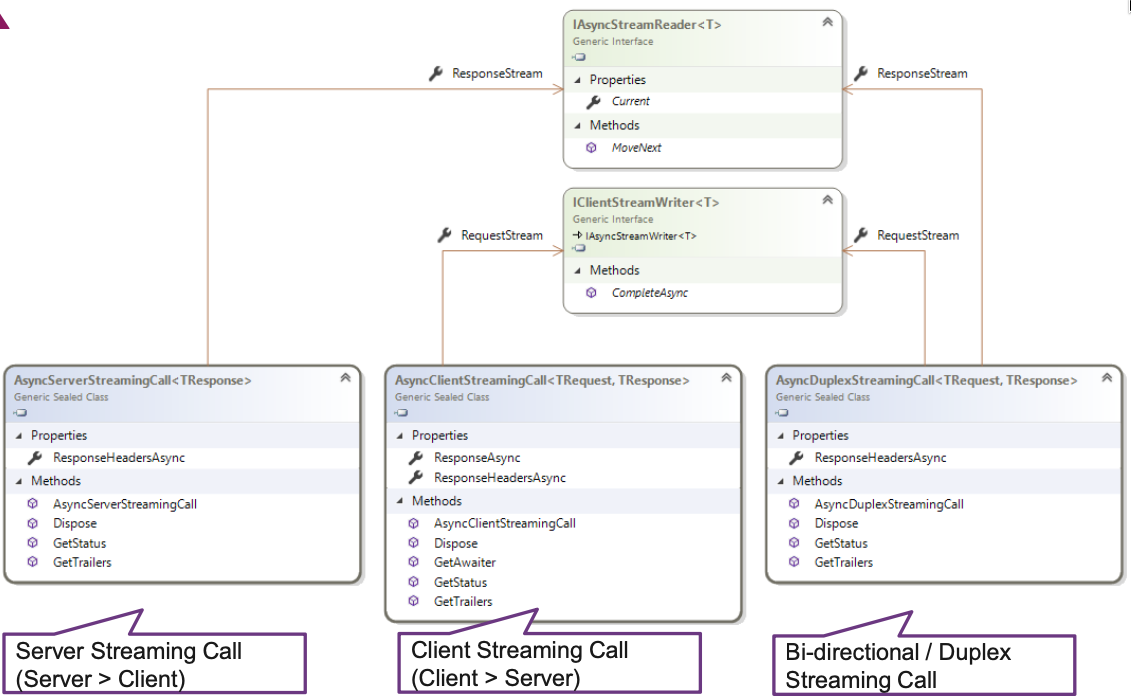
\includegraphics[width=\columnwidth]{streamapi}
\nfat{file\_streaming.proto}
\begin{lstlisting}
service FileStreamingService {
    //Server Streaming Call (Server > Client)
    rpc ReadFiles (google.protobuf.Empty) 
        returns (stream FileDto);
    //Client Streaming Call (Client > Server)
    rpc SendFiles (stream FileDto)
        returns (google.protobuf.Empty);
    //Bi-directional / Duplex Streaming Call
    rpc RoundtripFiles (stream FileDto)
        returns (stream FileDto);
}
message FileDto {
    string file_name = 1; 
    int32 line = 2; 
    string content = 3;
}
\end{lstlisting}
\subsubsection{Server Streaming Call}
Server stellt Files zur Verfügung und Client liest sie aus.
\nfat{Client Implementation:}
\begin{lstlisting}
                              //Call Object                    
using AsyncServerStreamingCall<FileDto> call = client.ReadFiles(new Empty()); //Leere Parameter

await foreach (FileDto file in call.ResponseStream.ReadAllAsync()) 
{
    WriteLine(\$"File: {file.FileName}, Line Nr: {file.Line}, Content: {file.Content}"); 
}
\end{lstlisting}
\fat{Service Implementation:}
\begin{lstlisting}
public override async Task ReadFiles(Empty request,
    IServerStreamWriter<FileDto> responseStream,
    ServerCallContext context)
{
    string[] files = Directory.GetFiles(@"..."); 
    foreach (string file in files)
    {
        string content; 
        int line = 0;
        using StreamReader reader = File.OpenText(file);
        while ((content = await reader.ReadLineAsync()) != null)
        {
            line++;
            FileDto reply = new() {
                FileName = file, 
                Line = line, 
                Content = content,
            };
        //Write to stream
        await responseStream.WriteAsync(reply);
     }
    } 
}
\end{lstlisting}
\subsubsection{Client Streaming Call}
Client stellt Files zur Verfügung und Server liest sie aus.
\nfat{Client Implementation:}
\begin{lstlisting}
                        //Payload-Type, Server reply
using AsyncClientStreamingCall<FileDto, Empty> call = client.SendFiles();

    string[] files = Directory.GetFiles(@"Files");
    foreach (string file in files)
{
    string content; 
    int line = 0;
    using StreamReader reader = File.OpenText(file);
    while ((content = await reader.ReadLineAsync()) != null) {
        line++;
        FileDto reply = new()
        {
            FileName = file, 
            Line = line, 
            Content = content, 
        };
        await call.RequestStream.WriteAsync(reply);
    } 
}
// Required!
await call.RequestStream.CompleteAsync(); // No more messages to come (server exits foreach-Loop) 
Empty result = await call; // Wait until service method is terminated / Get server reply
\end{lstlisting}
\fat{Service Implementation:}
\begin{lstlisting}
public override async Task<Empty> SendFiles( IAsyncStreamReader<FileDto> requestStream, ServerCallContext context)
{
    await foreach (FileDto message in requestStream.ReadAllAsync())
    {
        WriteLine(
            \$"File: {message.FileName}, Line Nr: {message.Line}, Line Content: {message.Content}");
    }
    return new Empty(); //Server reply 
}
\end{lstlisting}
\subsubsection{Bi-directional / Duplex Streaming Call}
Client empfängt Files vom Server, liest diese aus und schickt sie wieder zurück in diesem Beispiel:
\nfat{Client Implementation:}
\begin{lstlisting}
using AsyncDuplexStreamingCall<FileDto, FileDto> call = client.RoundtripFiles(); {
    // Read
    Task readTask = Task.Run(async () => //Run task, with no await
    {
        await foreach (FileDto message in call.ResponseStream.ReadAllAsync()) 
        {
            WriteLine(
                \$"File: {message.FileName}, Line Nr: {message.Line}, Line Content: {message.Content}");
        } 
    });
        
    // Write
   string[] files = Directory.GetFiles(@"Files");
   foreach (string file in files)
   {
        string content; int line = 0;
        using StreamReader reader = File.OpenText(file);
        while ((content = await reader.ReadLineAsync()) != null) {
            line++; 
            FileDto reply = new()
            {
                FileName = file, Line = line, Content = content, 
            };
           await call.RequestStream.WriteAsync(reply);
        } 
    }

    // Required!
    await call.RequestStream.CompleteAsync(); // No more messages to come (server exits foreach-Loop) 
    await readTask; // Wait until service method is terminated / all messages are received by client
}
\end{lstlisting}
\fat{Service Implementation:}
\begin{lstlisting}
public override async Task RoundtripFiles(
    IAsyncStreamReader<FileDto> requestStream, 
    IServerStreamWriter<FileDto> responseStream, 
    ServerCallContext context)
{
        await foreach (FileDto message in requestStream.ReadAllAsync())
        {
            //Write to stream
            await responseStream.WriteAsync(message);
            WriteLine(
                \$"File: {message.FileName}, Line Nr: {message.Line}, Line Content: {message.Content}");
        }
}
\end{lstlisting}
\subsection{Exception Handling}
Grundsätzlich immer via ''RpcException'' (basierend auf StatusCodes).
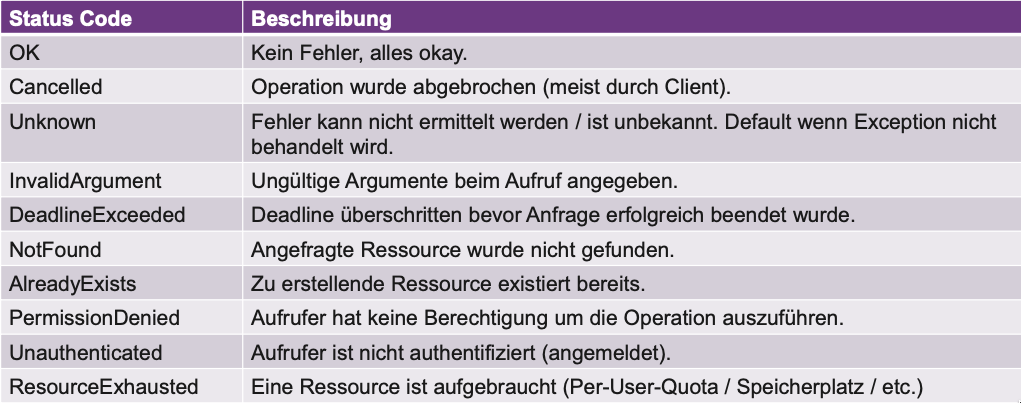
\includegraphics[width=\columnwidth]{statuscodes1}
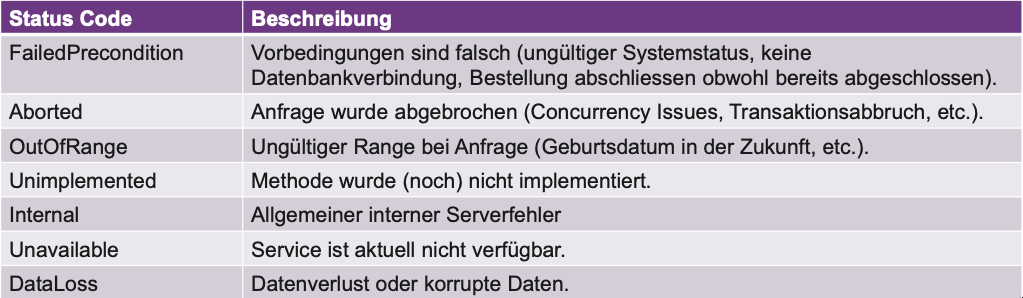
\includegraphics[width=\columnwidth]{statuscodes2}
\subsubsection{Common Mistakes}
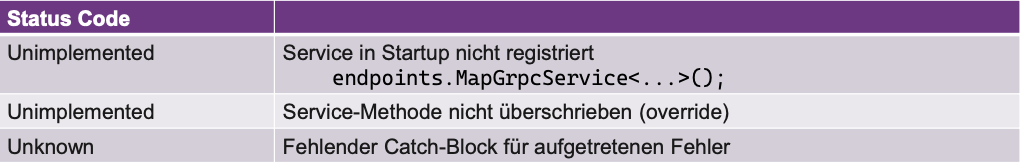
\includegraphics[width=\columnwidth]{commonmistakes}
\subsubsection{Unbehandelte Exception}
Exception wird auf Server nicht sauber behandelt.
\begin{itemize}
    \item Server Runtime fängt Exception
    \item Wirft RpcException
    \item Status Code “Unknown”
\end{itemize}
\begin{lstlisting}
public override Task<Empty> Unhandled(Empty request,
    ServerCallContext context)
    => throw new Exception("Unhandled Exception");
\end{lstlisting}
Ausgabe:
\begin{itemize}
    \item ex.Status.Code: Unknown
    \item ex.Status.Detail: Unhandled Exception
    \item ex.Trailers: <Leer>
\end{itemize}
\subsubsection{Behandelte Exception}
Exception wird auf Server sauber behandelt und korrekt verpackt.
\begin{lstlisting}
public override Task<Empty> NotFound(Empty request,
    ServerCallContext context)
    => throw new RpcException(
        new Status(StatusCode.NotFound, "Something was not found.") 
        );
\end{lstlisting}
Ausgabe:
\begin{itemize}
    \item ex.Status.Code: NotFound
    \item ex.Status.Detail: Something was not found.
    \item ex.Trailers: <Leer>
\end{itemize}
\subsubsection{Behandelte Exception mit Trailers}
Exception wird auf Server gefangen und korrekt verpackt
\begin{itemize}
    \item Metadata-Klasse verwenden
    \item Key-Value-Pair-Liste
    \item Binaries brauchen -bin als Suffix
\end{itemize}
\begin{lstlisting}
public override Task<Empty> Trailers(Empty request,
    ServerCallContext context)
    => throw new RpcException(
        new Status( StatusCode.NotFound, "Something was not found."),
        new Metadata
        {
            { "error-details",
              "Here are some more details..." },
            { "error-obj" +
              Metadata.BinaryHeaderSuffix,
              Encoding.UTF8.GetBytes("..payload..") }
        }
    );
\end{lstlisting}
Ausgabe:
\begin{itemize}
    \item ex.Status.Code: NotFound
    \item ex.Status.Detail: Something was not found.
    \item ex.Trailers: 2 Metadata-Entries
\end{itemize}
\subsubsection{Client-side Exception Handling}
\begin{itemize}
    \item Analog Serverseite: RpcException
    \item Kann (optional) mit when-Klausel auf verschiedene Catch-Blöcke verteilt werden
    \item RpcException umfassen auch alle Fehlersituationen bezüglich Kommunikation
    \begin{itemize}
        \item Endpoint antwortet nicht
        \item Verbindung bricht ab
    \end{itemize}
\end{itemize}
\begin{lstlisting}
try { /* ... */ }
// Communication exceptions
catch (RpcException e)
    when (e.StatusCode == StatusCode.Unavailable) {}
catch (RpcException e)
    when (e.StatusCode == StatusCode.NotFound) {}
catch (RpcException e)
    when (e.StatusCode == StatusCode.Aborted) {}
catch (RpcException e) {}
// Other stuff
catch (Exception) { /* ... */ }
\end{lstlisting}
Ausgabe:
\begin{itemize}
    \item ex.Status.Code: NotFound
    \item ex.Status.Detail: Something was not found.
    \item ex.Trailers: 2 Metadata-Entries
\end{itemize}

\end{multicols*}